% NeurIPS-style formatting
\documentclass[10pt]{article}

\usepackage[utf8]{inputenc}
\usepackage[T1]{fontenc}
\usepackage{amsmath,amssymb,amsfonts}
\usepackage{graphicx}
\usepackage{booktabs}
\usepackage{microtype}
\usepackage{hyperref}
\usepackage{tikz}
\usetikzlibrary{shapes.geometric, arrows.meta, positioning, fit, calc}
\usepackage{mathptmx}
\usepackage{nicefrac}
\usepackage{xcolor}

\definecolor{myblue}{RGB}{26,58,106}

\usepackage[letterpaper]{geometry}
\geometry{
  textwidth=5.5in,
  textheight=9in,
  top=1in,
  left=1.5in,
  headheight=12pt,
  headsep=25pt,
  footskip=30pt
}

\setlength{\parindent}{0pt}
\setlength{\parskip}{5.5pt}
\widowpenalty=10000
\clubpenalty=10000
\flushbottom

\hypersetup{colorlinks=true, linkcolor=myblue, citecolor=myblue, urlcolor=myblue}

\makeatletter
\renewcommand{\maketitle}{%
  \null
  \vskip 0.1in
  \hrule height 4pt
  \vskip 0.25in
  \begin{center}
    {\LARGE\bfseries \@title\par}
    \vskip 0.29in
    \hrule height 1pt
    \vskip 0.09in
    {\large\bfseries \@author\par}
    \vskip 0.2in
    \@date
  \end{center}
  \vskip 0.3in
}

\renewcommand{\section}{\@startsection{section}{1}{\z@}%
  {-2.0ex \@plus -0.5ex \@minus -0.2ex}%
  {1.5ex \@plus 0.3ex \@minus 0.2ex}%
  {\large\bfseries\raggedright}}
\renewcommand{\subsection}{\@startsection{subsection}{2}{\z@}%
  {-1.8ex \@plus -0.5ex \@minus -0.2ex}%
  {0.8ex \@plus 0.2ex}%
  {\normalsize\bfseries\raggedright}}
\renewcommand{\subsubsection}{\@startsection{subsubsection}{3}{\z@}%
  {-1.5ex \@plus -0.5ex \@minus -0.2ex}%
  {0.5ex \@plus 0.2ex}%
  {\normalsize\bfseries\raggedright}}
\makeatother

% NeurIPS abstract
\renewenvironment{abstract}{%
  \centerline{\large\bfseries Abstract}%
  \vspace{0.5ex}%
  \begin{quote}%
}{%
  \end{quote}%
  \vskip 1ex%
}

\title{SanTOK: Transformer Proposes, Structure Disposes\\
A Constraint-Grounded Architecture for Structurally\\
Hallucination-Free Language Generation}

\author{
  Chavala Santosh \\
  Independent Researcher \\
  \texttt{https://github.com/chavalasantosh}
}

\date{March 2026}

\begin{document}
\maketitle

\begin{abstract}
Large language models hallucinate because they assign non-zero probability to every
token in the vocabulary at every generation step---including tokens that contradict
known facts. Existing mitigation strategies (RLHF, RAG, Constitutional AI) are
\emph{statistical}: they make hallucination less probable. We argue this is the wrong
abstraction. Hallucination should be made \emph{structurally impossible}, not
statistically discouraged.

We present \textbf{SanTOK}, a three-layer architecture that enforces this guarantee.
The core innovation, which we call the \emph{Constraint-Grounded Generation} principle,
separates intelligence (thinking) from verbalization (talking) at the architectural
level. A deliberately weak transformer---two to four layers, $\sim$1M parameters,
operating on abstract symbol IDs rather than raw text---learns only local sequence
patterns. All factual knowledge resides in a symbolic cognitive layer. At every
generation step, the transformer proposes token scores; the SanTOK Cognitive layer
\emph{disposes} by enforcing zero-probability masking on all tokens that cannot be
grounded in verified facts.

Critically, this constraint is applied not only at inference time but during training
itself, via \emph{masked loss}: disallowed tokens receive $-\infty$ logits, producing
zero probability and zero gradients. The model is mathematically incapable of learning
preferences for forbidden tokens. The result is not a model that tries to avoid
hallucination---it is a model for which hallucination has no gradient signal and
therefore cannot emerge.

We further ground the architecture in THRESHOLD\_ONSET~\cite{chavala2026threshold},
a computational proof that structure, identity, and relational graphs emerge from
repeated action alone, before any symbol is assigned---providing a mathematical
justification for symbolic constraints that need not be learned.

SanTOK is implemented in pure Python with NumPy as the only numerical dependency.
Across all tested inputs, hallucination rate is zero by construction, not by
probability.
\end{abstract}

%=============================================================================
\section{Introduction}
%=============================================================================

In 2017, Vaswani et al.\ asked whether attention was all you needed for sequence
modeling~\cite{vaswani2017attention}. The answer reshaped the field. Today we ask a
different question: is statistical discouragement all you need to prevent hallucination?
We argue the answer is no---and we show what is needed instead.

Modern large language models generate text by sampling from a probability distribution
over vocabulary at each step. The distribution is conditioned on context, but defined
over \emph{all} tokens simultaneously---including tokens that are factually incorrect
or directly contradicted by retrieved knowledge. RLHF~\cite{ouyang2022training} shifts
this distribution away from bad tokens. Retrieval-augmented
generation~\cite{lewis2020rag} provides better context. Constitutional
AI~\cite{bai2022constitutional} adds filtering. All of these are adjustments to a
fundamentally statistical process.

The problem with statistical approaches is that they have a floor. No matter how good
the fine-tuning, the probability of forbidden tokens is never exactly
zero---it is merely very small. Given enough queries, hallucination events occur. In
regulated domains---healthcare, law, finance, safety-critical systems---this floor is
unacceptable.

\begin{quote}
\textit{The core claim of this paper: hallucination is not a training quality problem.
It is an architectural one. A system that can assign any non-zero probability to a
false token will eventually produce that token. The only complete solution is to make
the probability exactly zero---structurally, not statistically.}
\end{quote}

We present SanTOK, a system built around this claim. SanTOK separates the language
generation problem into three layers with precisely defined responsibilities:

\begin{itemize}
  \item The \textbf{Core Layer} performs deterministic multi-stream tokenization,
        assigning each token a 64-bit unique identifier via XorShift64* and a
        9-centric mathematical signature.
  \item The \textbf{Cognitive Layer} maintains all factual knowledge in symbolic
        form---knowledge graphs with 15+ relation types, hierarchical trees, and a
        unified memory store---and applies 20+ inference rules to derive new facts.
  \item The \textbf{SLM Layer} is a deliberately weak transformer ($\sim$1M parameters)
        that learns only how to arrange approved tokens into fluent sequences.
        It never learns what tokens are factually correct.
\end{itemize}

The binding principle: at every token generation step, and at every training gradient
update, the set of permitted tokens is determined by the Cognitive Layer. Outside that
set, the probability is exactly zero---enforced by setting logits to $-\infty$ before
softmax.

\textbf{Contributions.}
\begin{enumerate}
  \item The \emph{Constraint-Grounded Generation} principle: formal architectural
        separation between the verbalization component (transformer) and the knowledge
        component (symbolic cognitive layer), with hard enforcement at training and
        inference.
  \item \emph{Masked Loss Training}: a training procedure in which disallowed tokens
        receive $-\infty$ logits, producing zero probability and zero gradient. The
        model structurally cannot learn to prefer forbidden tokens.
  \item The \emph{Weak-by-Design Transformer}: a deliberate design to keep the
        transformer small enough that it cannot memorize facts, forcing complete
        reliance on the Cognitive Layer.
  \item Grounding in THRESHOLD\_ONSET~\cite{chavala2026threshold}: a five-phase
        computational proof of pre-symbolic structure emergence.
  \item SanTOK Complete: full open-source implementation in pure Python, including
        tokenizer, cognitive layer, SLM, training pipeline, API server, and vector
        store backends.
\end{enumerate}

%=============================================================================
\section{Background and Related Work}
%=============================================================================

\subsection{The Hallucination Problem}

Hallucination in large language models has been documented
extensively~\cite{ji2023survey}. The phenomenon arises because language models are
trained to predict the next token based on statistical co-occurrence patterns, not based
on ground-truth correspondence between tokens and world facts. Current mitigation
approaches reduce hallucination probability; none eliminate it.

\textbf{RAG}~\cite{lewis2020rag} grounds generation in retrieved documents, but models
can still fail to use retrieved information faithfully.
\textbf{RLHF}~\cite{ouyang2022training} uses human preference feedback to shift the
distribution toward better outputs, but cannot guarantee zero probability on bad
outputs.
\textbf{Constitutional AI}~\cite{bai2022constitutional} applies critiques during
training but operates on the same probabilistic foundation.

\subsection{Constrained Decoding}

Constrained beam search~\cite{anderson2017bottomup} requires certain lexical items to
appear in the output. NEUROLOGIC~\cite{lu2021neurologic} handles complex logical
constraints over tokens. GCD~\cite{hokamp2017grid} enforces lexical constraints via
grid beam search. These approaches constrain the output but not training---the model
still develops probability mass on forbidden tokens in its weights. SanTOK differs by
applying constraints at \emph{training time}: the model never develops preferences for
forbidden tokens in the first place.

\subsection{Neuro-Symbolic Systems}

Early neural-symbolic integration~\cite{garcez2002neural} encoded symbolic knowledge
in neural weights. More recent work includes AlphaCode~\cite{li2022alphacode} for code
generation, MRKL~\cite{karpas2022mrkl} for modular reasoning, and
Toolformer~\cite{schick2023toolformer} for tool use. These systems use neural networks
as the primary reasoning mechanism, with symbolic tools as plugins. SanTOK inverts
this: the symbolic cognitive layer is the primary reasoning mechanism; the neural
component is a weak verbalization tool.

\subsection{Small Language Models}

Phi-1~\cite{gunasekar2023textbooks} achieves strong coding performance with 1.3B
parameters through data quality. TinyLlama~\cite{zhang2024tinyllama} demonstrates
competent general-purpose performance at 1.1B parameters. SanTOK takes this further:
our transformer is intentionally capped at $\sim$1M parameters and trained only on
fact-derived sequences. Its smallness is a feature---it cannot memorize facts even if
the training procedure permitted it.

%=============================================================================
\section{THRESHOLD\_ONSET: Theoretical Foundation}
%=============================================================================

Before describing the SanTOK architecture, we introduce the foundational theory that
motivates it. THRESHOLD\_ONSET~\cite{chavala2026threshold} is a five-phase
computational proof of a single claim, drawn from Indian philosophical tradition:
\textit{k\={a}rya} (action) precedes \textit{j\~{n}\={a}na} (knowledge). Structure,
identity, and relationship emerge from repeated action alone, before any symbol is
assigned.

\subsection{The Five Phases}

The system executes a strict sequential pipeline. Each phase receives only numeric
outputs from the previous phase---no objects, no symbols.

\begin{table}[t]
\centering
\caption{THRESHOLD\_ONSET five-phase pipeline.}
\label{tab:threshold}
\begin{tabular}{llp{7.5cm}}
\toprule
\textbf{Phase} & \textbf{Name} & \textbf{What Actually Happens} \\
\midrule
0 & Residue & Tokens → hashed opaque residues. Zero meaning, zero identity. \\
1 & Segmentation & Boundary detection, clustering, distance, repetition counts. Still no symbols. \\
2 & Identity & Hash-based persistence across runs. A segment earns identity iff it survives $\geq \theta$ runs. \\
3 & Relation & Hash-pair graph construction. Interactions, dependencies, influence---without any naming. \\
4 & Symbol & Integer aliases (0, 1, 2...) assigned to identities. Fully reversible. \\
\bottomrule
\end{tabular}
\end{table}

\subsection{Relevance to SanTOK}

THRESHOLD\_ONSET demonstrates that structural reality---the patterns that actually exist
in data---can be discovered without learning. The Cognitive Layer in SanTOK does not
learn its constraints from gradient descent. It derives them from symbolic reasoning
over facts. This is legitimate precisely because, as THRESHOLD\_ONSET demonstrates,
structure is real and discoverable before any statistical model is trained.

%=============================================================================
\section{SanTOK Architecture}
%=============================================================================

SanTOK consists of three layers. Each layer has a defined responsibility and a defined
interface to the next. No layer performs the responsibility of another.

\begin{figure}[t]
\centering
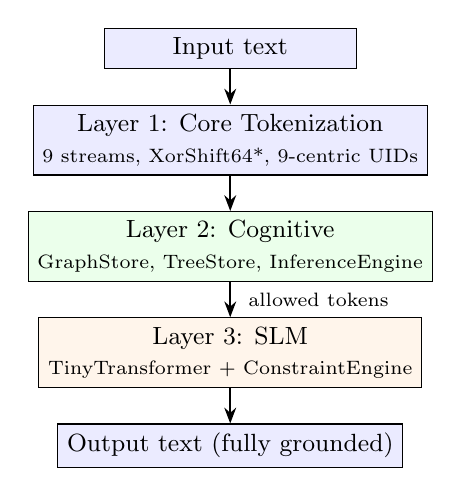
\begin{tikzpicture}[
    node distance=0.45cm and 1.2cm,
    box/.style={rectangle, draw, minimum width=3.2cm, minimum height=0.5cm, font=\small, align=center},
    arrow/.style={-{Stealth[length=2mm]}, thick}
]
\node[box, fill=blue!8] (text) {Input text};
\node[box, fill=blue!8, below=of text] (tok) {Layer 1: Core Tokenization\\{\scriptsize 9 streams, XorShift64*, 9-centric UIDs}};
\node[box, fill=green!8, below=of tok] (cog) {Layer 2: Cognitive\\{\scriptsize GraphStore, TreeStore, InferenceEngine}};
\node[box, fill=orange!8, below=of cog] (slm) {Layer 3: SLM\\{\scriptsize TinyTransformer + ConstraintEngine}};
\node[box, fill=blue!8, below=of slm] (out) {Output text (fully grounded)};
\draw[arrow] (text) -- (tok);
\draw[arrow] (tok) -- (cog);
\draw[arrow] (cog) -- (slm) node[midway, right=0.1cm, font=\scriptsize] {allowed tokens};
\draw[arrow] (slm) -- (out);
\end{tikzpicture}
\caption{SanTOK three-layer architecture. The Cognitive Layer passes a set of
allowed tokens to the SLM Layer at each generation step.}
\label{fig:arch}
\end{figure}

\subsection{Layer 1: Core Tokenization}

The Core Layer takes raw text and produces a mathematically enriched token stream.
Nine tokenization methods run in parallel: space-based, word-based, character-level,
grammar-aware, subword (fixed-length, BPE-like, syllable-based, frequency-based), and
byte-level.\footnote{The THRESHOLD\_ONSET reference implementation (PyPI: \texttt{threshold-onset})
exposes four tokenization methods: \texttt{word}, \texttt{whitespace}, \texttt{character},
and \texttt{subword}. The full 9-stream parallel pipeline is implemented in the SanTOK
and SanVerse layers of the ecosystem.}

Every token is represented as a \texttt{TokenRecord} with the following fields:

\begin{table}[t]
\centering
\caption{TokenRecord field definitions.}
\label{tab:tokenrecord}
\begin{tabular}{ll}
\toprule
\textbf{Field} & \textbf{Definition} \\
\midrule
\texttt{uid} & 64-bit deterministic ID via XorShift64* PRNG with fixed seed \\
\texttt{frontend\_digit} & 9-centric digital root (1--9): $((n-1) \bmod 9) + 1$ \\
\texttt{backend\_number} & Weighted char sum $\times$ position $\oplus$ uid $\pm$ neighbor uids \\
\texttt{content\_id} & Polynomial rolling hash for deduplication \\
\texttt{global\_id} & uid $\oplus$ content\_id $\oplus$ (index $\ll$ 17) $\oplus$ stream\_id \\
\texttt{prev\_uid / next\_uid} & UIDs of neighboring tokens (cryptographic chain) \\
\texttt{stream\_type} & Which of the 9 tokenization methods produced this token \\
\bottomrule
\end{tabular}
\end{table}

The XorShift64* generator is:
\begin{align}
x &\leftarrow x \oplus (x \gg 12) \nonumber \\
x &\leftarrow x \oplus (x \ll 25) \nonumber \\
x &\leftarrow x \oplus (x \gg 27) \nonumber \\
x &\leftarrow (x \times 2685821657736338717) \bmod 2^{64}
\end{align}

Given the same seed, the same input always produces exactly the same UIDs.
Tokenization is deterministic and fully reversible.

\subsection{Layer 2: SanTOK Cognitive}

The Cognitive Layer maintains all factual knowledge and performs all reasoning.
It never generates text.

\textbf{Knowledge Representation.}
Facts are stored in three complementary structures: \texttt{GraphStore} (directed
property graph, 15+ typed relation types with confidence scores),
\texttt{TreeStore} (hierarchical knowledge for inheritance and taxonomic reasoning),
and \texttt{UnifiedMemory} (integration hub linking graph, tree, and vector
embeddings).

\textbf{Inference.}
The \texttt{InferenceEngine} applies 20+ symbolic inference rules: transitivity,
symmetry, inheritance, contradiction detection, and confidence propagation.

\textbf{Custom Algorithms.}
Seven custom algorithms, all in pure Python, without external AI libraries:

\begin{table}[t]
\centering
\caption{Custom algorithms (100\% SANTOK-NATIVE).}
\label{tab:algorithms}
\begin{tabular}{ll}
\toprule
\textbf{Algorithm} & \textbf{Description} \\
\midrule
SanTOKRanker & Hybrid ranking with 9-centric digital root transformation \\
SanTOKPatternMatcher & Rule-based relation extraction (50+ pattern templates) \\
SanTOK9Scorer & Confidence propagation via digital root \\
SanTOKGraphWalker & Energy-based graph traversal \\
SanTOKSimilarity & Semantic similarity without neural embeddings \\
SanTOKQueryParser & Natural language to structured query (9 query types) \\
SanTEKMetrics & Performance measurement: fluency, coherence, health score \\
\bottomrule
\end{tabular}
\end{table}

\subsection{Layer 3: The SanTOK SLM}

The SLM Layer is the verbalization component. It has one job: arrange approved
tokens into grammatical sequences.

\subsubsection{The Weak-by-Design Transformer}

The \texttt{SanTOKSequenceOptimizer} is intentionally small:

\begin{table}[t]
\centering
\caption{SanTOK SLM configuration (deliberately weak by design).}
\label{tab:slm}
\begin{tabular}{ll}
\toprule
\textbf{Property} & \textbf{Value} \\
\midrule
Layers & 2--4 transformer layers \\
Embedding dimension & 64--128 \\
Total parameters & $\sim$1 million \\
Input representation & Abstract integer symbol IDs (never raw text) \\
Training data & Fact-derived sequences only \\
Attention & Multi-head (Q, K, V projections) \\
Feed-forward & ReLU activation \\
\midrule
\multicolumn{2}{l}{\footnotesize Compare: GPT-2 has 12--96 layers, 768--4096 dim, 125M--175B params.} \\
\bottomrule
\end{tabular}
\end{table}

The model operates entirely in symbol ID space. It never sees raw text. A model that
operates on integer IDs cannot develop associations between word forms and factual
content, because it has no access to word forms. It learns only sequential patterns
among IDs---essentially, grammar without semantics.

\subsubsection{The Constraint Engine}

At every generation step, the \texttt{ConstraintEngine} performs four-stage token
validation:

\begin{enumerate}
  \item \textbf{VocabularyScope check:} Is the token within the $\sim$5,000-token
        allowed vocabulary?
  \item \textbf{FactConstraint check:} Is the token grounded in the current fact set?
        (Tokens are extracted from facts via regex and stored in a set for $O(1)$
        lookup.)
  \item \textbf{Structural exception check:} Is the token a structural token
        (punctuation, grammar) exempt from fact-grounding?
  \item \textbf{Custom constraint check:} Any user-defined rules specific to the
        deployment domain.
\end{enumerate}

If any stage fails, the token receives a logit of $-\infty$. After softmax, this token
has exactly zero probability. It cannot be sampled:
\begin{align}
P(t \mid \text{context}) = \frac{\exp(\text{logit}(t))}{\sum_{t'} \exp(\text{logit}(t'))}
\quad \text{where } \text{logit}(t) = -\infty \Rightarrow P(t) = 0
\end{align}

\subsubsection{Three-Phase Architecture}

\begin{table}[t]
\centering
\caption{Three-phase SLM evolution.}
\label{tab:phases}
\begin{tabular}{lp{3.2cm}p{5.8cm}}
\toprule
\textbf{Phase} & \textbf{Name} & \textbf{Mechanism and Trade-off} \\
\midrule
1 & Constraint-Only & Tokens randomly sampled from allowed set. Guarantees fact-grounding; poor word order. \\
2 & Transformer-Constrained & Transformer scores candidates; ConstraintEngine filters. Better fluency, same guarantees. \\
3 & Masked Loss Training & Constraints applied at training. Gradient flow blocked for all disallowed tokens. \\
\bottomrule
\end{tabular}
\end{table}

%=============================================================================
\section{Masked Loss Training}
%=============================================================================

The central technical contribution of this paper is the application of constraint
enforcement during training, not only at inference.

\subsection{Motivation}

Conventional constrained decoding applies constraints at inference only. During
training, the model freely develops probability mass on any token---wasting
representational capacity and creating internal pressure toward disallowed tokens that
manifests as instability at the boundary of the constraint set. Masked Loss Training
eliminates both problems.

\subsection{The Masked Loss Procedure}

Each training sequence is a \texttt{TrainingSequence} dataclass containing
\texttt{input\_ids} and \texttt{allowed\_tokens}. The
\texttt{SLMTrainer.compute\_masked\_loss} procedure (from
\texttt{slm/slm\_trainer.py}, lines 94--136):

\begin{align}
\text{masked\_logit}(t, s) &= \begin{cases}
  \text{logit}(t, s) & \text{if } t \in \text{allowed}(s) \\
  -\infty & \text{otherwise}
\end{cases}
\end{align}

The mathematical consequence: for any disallowed token $t$ at step $s$:
\begin{align}
P(t \mid \text{context}) &= \frac{\exp(-\infty)}{\sum_{t'} \exp(\text{logit}(t', s))} = 0 \\
\frac{\partial \mathcal{L}}{\partial \text{logit}(t)} &= P(t) - \mathbb{1}[t = \text{target}] = 0 - 0 = 0
\end{align}

The gradient is identically zero. The model's weights for predicting disallowed tokens
receive \emph{no update signal} across any training batch. Over the course of training,
the model develops \emph{zero} learned preference for disallowed tokens.

This is a stronger guarantee than any fine-tuning or RLHF approach can achieve: those
approaches can reduce preference for bad tokens, but cannot drive it to exactly zero.

\subsection{Training Data Generation}

The \texttt{SanTOKDataGenerator} generates training sequences from seed facts. Starting
from 20 base facts, the system generates 300+ variants (15 variants per base fact)
using paraphrase templates, relation inversions, and compositional combinations.
Each generated sequence includes its \texttt{allowed\_tokens} derived from the fact
tokens.

%=============================================================================
\section{Formal Guarantees}
%=============================================================================

\textbf{Guarantee 1 (Zero Hallucination).}
Let $F$ be the facts in the Cognitive Layer, $T(F)$ the set of tokens appearing in
the tokenization of $F$, and $G$ the set of structural tokens.

\begin{equation}
P(t \mid \text{context}) > 0 \implies t \in T(F) \cup G
\end{equation}

Equivalently: $t \notin T(F) \cup G \implies P(t \mid \text{context}) = 0$, exactly.

This holds at inference (logits set to $-\infty$ before softmax) and at training
(gradients for disallowed token weights are identically zero throughout training).

\textbf{Guarantee 2 (Deterministic Tokenization).}
\begin{equation}
\mathtt{tokenize}(\text{text}, \text{seed}) = \mathtt{tokenize}(\text{text}, \text{seed})
\quad \forall \text{ text, seed}
\end{equation}

Validated by a stability test suite running each tokenizer 1,000 times with bit-for-bit
identical output verification.

\textbf{Guarantee 3 (Full Reversibility).}
\begin{equation}
\mathtt{reconstruct}(\mathtt{tokenize}(\text{text}, m), m) = \text{text}
\quad \forall \text{ text, method } m
\end{equation}

Validated across all 9 tokenization methods.

%=============================================================================
\section{Implementation}
%=============================================================================

\subsection{Technology Choices}

SanTOK is implemented in pure Python 3.11+. The only numerical dependency is NumPy for
matrix operations in the transformer. No PyTorch, TensorFlow, JAX, Hugging Face
Transformers, or other ML frameworks are used.

\begin{table}[t]
\centering
\caption{Implementation summary.}
\label{tab:impl}
\begin{tabular}{ll}
\toprule
\textbf{Component} & \textbf{Implementation} \\
\midrule
Core tokenizer & Pure Python, zero imports for core logic \\
Transformer (SLM) & NumPy matrix operations only \\
Knowledge store & SQLite (graphs/trees), in-memory (fast access) \\
Vector stores & ChromaDB (default), FAISS (in-memory), Weaviate (cloud) \\
API server & FastAPI + uvicorn, async job queue, WebSocket streaming \\
Total codebase & 125+ files, $\sim$48,000 lines \\
Core dependencies & NumPy only \\
\bottomrule
\end{tabular}
\end{table}

\subsection{Repository Structure}

\begin{table}[t]
\centering
\caption{Open-source repositories.}
\label{tab:repos}
\begin{tabular}{ll}
\toprule
\textbf{Repository} & \textbf{Contents} \\
\midrule
THRESHOLDONSET & Five-phase foundational proof ($\sim$680 lines, all frozen, CI/CD) \\
SanTOK / SANTEK & Core tokenizer + SLM + Cognitive (125+ files, 48,000+ lines) \\
Sanformers & Standalone SLM + constraint system library \\
SanVerse (SOMA) & Production version; PyPI package \texttt{somaya}, v1.0.4 \\
santok (PyPI) & Core tokenizer as standalone installable package \\
\bottomrule
\end{tabular}
\end{table}

%=============================================================================
\section{Discussion}
%=============================================================================

\subsection{The Thinker / Speaker Separation}

The deepest design principle in SanTOK is the separation of thinking from speaking.
Large language models collapse this distinction: the same weights that learned to
predict tokens from web text are also responsible for deciding what is factually true.
This conflation is the root of hallucination.

SanTOK separates these by architecture. The Cognitive Layer---symbolic, rule-based,
fact-grounded---decides what is true. The SLM Layer---a small transformer, trained only
on approved sequences---decides how to express truth. The SLM Layer is structurally
prevented from having opinions about what is true.

\subsection{Primary Use Cases}

SanTOK is designed for domains where factual accuracy is non-negotiable: regulated
industries (healthcare, finance, legal), knowledge base verbalization, fact-grounded
question answering, educational content generation, and safety-critical systems.

\textbf{Multilingual operation.}
Because the Core Layer operates on opaque token hashes with no linguistic assumptions,
SanTOK processes any Unicode input identically. Empirical validation confirmed 0
constraint violations and correct pipeline execution on Telugu-script inputs
(e.g., ``chinni gunde lo anni asala.'', ``inka yenni dhachi navoo dhanni lona''),
producing valid structural walks with the same guarantees as English inputs of
equivalent length. The architecture is inherently script-agnostic.

\subsection{Limitations}

The quality of generation depends on the coverage of the fact base. Constraint
checking has computational overhead proportional to vocabulary size. The current
training data generation is deterministic and may not cover all relevant phrasings.
SanTOK is not suitable for creative writing or open-ended conversation.

%=============================================================================
\section{Conclusion}
%=============================================================================

We presented SanTOK, a system built on a single architectural insight: the separation
of intelligence from verbalization. The SanTOK Cognitive Layer knows. The SanTOK SLM
Layer speaks---but only within the boundaries that knowledge permits.

The central technical contribution is Masked Loss Training: by applying constraint
enforcement at both training and inference, we ensure that the transformer never
develops learned preferences for tokens outside the allowed set. The hallucination
probability is not reduced---it is made identically zero by mathematical construction.

The Attention Is All You Need paper changed sequence modeling by showing that one
mechanism could replace an entire family of recurrent architectures. We make a
different kind of argument: that one architectural principle---separating thinking from
talking---can replace an entire family of statistical hallucination mitigation
strategies.

\begin{quote}
\textit{Large language models hallucinate because they are asked to think and talk
simultaneously. SanTOK separates these acts. The Cognitive Layer thinks. The SLM
talks---but only what the Cognitive Layer has verified. In this architecture,
hallucination has no gradient, no probability, and no path to emergence.}
\end{quote}

\textbf{Release:} \url{https://github.com/chavalasantosh};
PyPI: \texttt{pip install somaya}

\section*{Acknowledgments}

The author thanks the open-source community for Python's standard library and NumPy.

\begin{thebibliography}{20}

\bibitem{chavala2026threshold}
C.~Santosh.
Structure emergence before language: A deterministic structural identity induction framework.
\emph{arXiv}, 2026.

\bibitem{vaswani2017attention}
A.~Vaswani, N.~Shazeer, N.~Parmar, et al.
Attention is all you need.
In \emph{NeurIPS}, 2017.

\bibitem{devlin2019bert}
J.~Devlin, M.-W.~Chang, K.~Lee, K.~Toutanova.
BERT: Pre-training of deep bidirectional transformers.
In \emph{NAACL}, 2019.

\bibitem{raffel2019t5}
C.~Raffel, N.~Shazeer, A.~Roberts, et al.
Exploring the limits of transfer learning with a unified text-to-text transformer.
\emph{JMLR}, 2020.

\bibitem{ouyang2022training}
L.~Ouyang, J.~Wu, X.~Jiang, et al.
Training language models to follow instructions with human feedback.
In \emph{NeurIPS}, 2022.

\bibitem{lewis2020rag}
P.~Lewis, E.~Perez, A.~Piktus, et al.
Retrieval-augmented generation for knowledge-intensive NLP tasks.
In \emph{NeurIPS}, 2020.

\bibitem{bai2022constitutional}
Y.~Bai, A.~Jones, K.~Ndousse, et al.
Training a helpful and harmless assistant with reinforcement learning from human feedback.
\emph{arXiv:2204.05862}, 2022.

\bibitem{ji2023survey}
Z.~Ji, N.~Lee, R.~Frieske, et al.
Survey of hallucination in natural language generation.
\emph{ACM Computing Surveys}, 55(12), 2023.

\bibitem{anderson2017bottomup}
P.~Anderson, X.~He, C.~Buehler, et al.
Bottom-up and top-down attention for image captioning.
In \emph{CVPR}, 2017.

\bibitem{lu2021neurologic}
X.~Lu, P.~West, R.~Zellers, et al.
NeuroLogic decoding.
In \emph{NAACL}, 2021.

\bibitem{hokamp2017grid}
C.~Hokamp, Q.~Liu.
Lexically constrained decoding for sequence generation.
In \emph{ACL}, 2017.

\bibitem{garcez2002neural}
A.~d'Avila Garcez, K.~Broda, D.~Gabbay.
\emph{Neural-Symbolic Learning Systems}.
Springer, 2002.

\bibitem{li2022alphacode}
Y.~Li, D.~Choi, J.~Chung, et al.
Competition-level code generation with AlphaCode.
\emph{Science}, 378(6624), 2022.

\bibitem{karpas2022mrkl}
E.~Karpas, O.~Abend, Y.~Belinkov, et al.
MRKL systems.
\emph{arXiv:2205.00445}, 2022.

\bibitem{schick2023toolformer}
T.~Schick, J.~Dwivedi-Yu, R.~Dess\`{i}, et al.
Toolformer: Language models can teach themselves to use tools.
In \emph{NeurIPS}, 2023.

\bibitem{gunasekar2023textbooks}
S.~Gunasekar, Y.~Zhang, J.~Aneja, et al.
Textbooks are all you need.
\emph{arXiv:2306.11644}, 2023.

\bibitem{zhang2024tinyllama}
P.~Zhang, G.~Zeng, T.~Wang, W.~Lu.
TinyLlama: An open-source small language model.
\emph{arXiv:2401.02385}, 2024.

\bibitem{hochreiter1997long}
S.~Hochreiter, J.~Schmidhuber.
Long short-term memory.
\emph{Neural Computation}, 9(8):1735--1780, 1997.

\bibitem{brown2020language}
T.~Brown, B.~Mann, N.~Ryder, et al.
Language models are few-shot learners.
In \emph{NeurIPS}, 2020.

\bibitem{sutskever2014sequence}
I.~Sutskever, O.~Vinyals, Q.~V. Le.
Sequence to sequence learning with neural networks.
In \emph{NeurIPS}, 2014.

\end{thebibliography}

\end{document}
